\documentclass[a4paper]{article}

\usepackage{amsmath}
\usepackage{amssymb}
\usepackage{graphicx}
\usepackage[hidelinks]{hyperref}
\usepackage{listings}
\newtheorem{proposition}{Proposition}
\DeclareMathOperator{\sgn}{\mathrm{sgn}}
\DeclareMathOperator{\trunc}{\mathrm{trunc}}
\lstset{
    basicstyle=\small\tt,
    numbers=left
}

\title{The simplest algorithm to convert a floating-point number into the sum of two square roots}
\author{Jason Zheng}

\begin{document}
\maketitle

\section{Introduction}
Some numerical calculators will return mathematical expressions of the form $\dfrac{\pi}{3}$ or $\dfrac{2\sqrt{2}}{3}$ instead of floating-point numbers when calculating fractions and radicals, and can also display $1+\sqrt{2}$ and $\dfrac{\sqrt{2}+\sqrt{3}}{2}$. The first two can be derived in almost an instant by simple arithmetic, but the last two involve addition operations. If we want to find the values of $a,b,c$ in $\dfrac{\sqrt{a}+\sqrt{b}}{c}$ separately, the most straightforward way is to use 3 for-loops. But this is very inefficient. How can we reduce the use of loops and increase efficiency? That's what I wrote this article for: to introduce a new algorithm to convert a floating-point number into the sum of two square roots.

\section{Theory}
We start with the form without the denominator. To reduce repetition, first define a function\[S(x,y)=\sgn(x)\sqrt{|x|}+\sgn(y)\sqrt{|y|} \quad\text{for } x,y\in\mathbb{Z}\]If only the floating-point number $n=S(a,b)$ is known, some mathematical tricks can be used and just use a while loop to find $a$ and $b$, instead of using a double for loop. In short, we are trying to find $S^{-1}(x)$.

First of all, it is impossible to compute $S^{-1}(x)$ using the specified formula, too much information is already lost in floating-point numbers. Using the exhaustive method becomes the only way, but which method to use and which starting value to set is a matter of discussion. The first one I have already explained before, and the second one will be discussed next, starting with the following true proposition
\begin{proposition}
    There is a sum of two numbers $a+b$ and $c=\dfrac{a+b}{2}$, then $|c-a|=|c-b|$.
\end{proposition}

According to the proposition, there is $n=S(a,b)$, and we can search from $\dfrac{n}{2}$ in the direction of $+\infty$ or $-\infty$, and as soon as $a$ is located there can be a unique $b$, and another conditional judgment can determine whether they are the desired ones.

Of course, it is not appropriate to take $\dfrac{n}{2}$ as the starting value, we require two integers, to truncate the tail after rounding $\left(\dfrac{n}{2}\right)^2$ as the starting value is more appropriate.

However, consider $\left(\dfrac{\sqrt{100}+\sqrt{101}}{2}\right)^2\approx100.499$, which is truncated to 100, and there is an omission in this design. However, there is the following limit \[\lim_{x\to+\infty} \left(\frac{\sqrt{x}+\sqrt{x+1}}{2}\right)^2 - x=\frac{1}{2}\] which shows that the function $f(x)=\left(\dfrac{\sqrt{x}+\sqrt{x+1}}{2}\right)^2$ can be approximated as $x+\dfrac{1}{2}$, and the error is already less than $1\%$ when $x>5.76$.

In this way, we can find the two numbers in the root sign even if they are close to each other.

From the above analysis, we can set the starting value
\[
    start(n)=
    \begin{cases}
        \trunc(\frac{n}{2})^2+\frac{1}{2}  & \text{if }n>0 \\
        -\trunc(\frac{n}{2})^2-\frac{1}{2} & \text{if }n<0
    \end{cases}
\]

In the following, for writing convenience, the square root of a negative number is considered to be the square root of its absolute value multiplied by -1.

Knowing that $n=S(a,b)$, after setting the starting value $start$, let $step=0.5$ and find an endpoint \[\alpha=start-step\] then we can calculate the other endpoint \[\beta=\frac{n}{2}-|\sqrt{a}-\frac{n}{2}|\] Since $\beta $ must be an integer, it is also necessary to do the following \[\beta=\sqrt{\sgn(\beta)\mathrm{round}(\beta^2)}\] where \verb|round| means rounded to the nearest integer.

If $\sqrt{\alpha}+\sqrt{\beta}=n$, then $\alpha$ and $\beta$ are the required $a$ and $b$. Otherwise make $step\pm1$ and keep looking in the direction of positive or negative infinity.

\section{Implementation}
The following example uses the Python standard library, or you can also use libraries like \verb|mpmath| to improve precision.

\begin{lstlisting}[language=python, name=example1]
import math

def num2sqrts(n, max_num=1000):
	if n >= 0:
        mid = math.floor((n / 2) ** 2) + 0.5
    elif n < 0:
        mid = math.ceil(-(n / 2) ** 2) - 0.5
    fsqrt = lambda n: math.copysign(math.sqrt(math.fabs(n)), n)
    actual_mid = n / 2
    t = 0.5
    while True:
        a = fsqrt(mid + t)
        d = math.fabs(a - actual_mid)
        b = actual_mid - d
        b = fsqrt(math.copysign(round(b ** 2), b))
\end{lstlisting}
In theory, the algorithm can keep running until it finds the right value. However, considering the practical situation, the stopping condition still needs to be set.
\begin{lstlisting}[language=python, name=example1]
        if abs(a ** 2) > max_num or abs(b ** 2) > max_num:
            return
        if math.isclose(a + b, n):
            return int(round(math.copysign(a ** 2, a))), \
                int(round(math.copysign(b ** 2, b)))
        t += 1
\end{lstlisting}
Finally, function \verb|num2sqrts| returns tuples of length 2. If the return value is \verb|None|, then the right value isn't found.

\begin{figure}[htb]
    \centering
    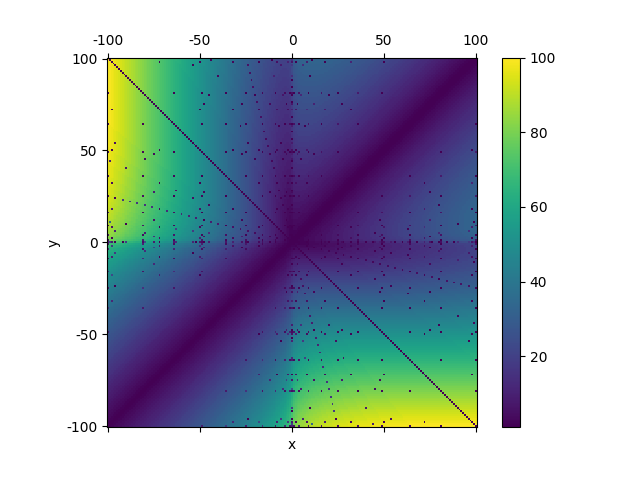
\includegraphics[width=0.8\linewidth]{perform1.pdf}
    \caption{Perform of this algorithm}
    \label{fig:perform1}
\end{figure}

To show the performance of this algorithm, I take$-100\leq x\leq100$ and $-100\leq y\leq100$, then calculate the number of cycles needed to find $x$ and $y$ in $S(x,y)$, and mark them with different colors. So, Figure \ref{fig:perform1} is drawn. It can be seen that as the difference between x and y gets larger, it takes longer.

But when we execute the following (or similar) lines
\begin{lstlisting}[language=python]
num2sqrts(2 * math.sqrt(123))
\end{lstlisting}
it returns \verb|(492, 0)|. The loop is executed 438 times. But the value $2\sqrt{123}$ can be found by a simpler method. So I assign all the values on the diagonal of the first and third quadrants to 1.

At the end, I will explain what to do if a denominator is added. It would be too inefficient to find a new algorithm, and we can completely exhaust the denominator.
\begin{lstlisting}[language=python, name=example2]
def num2sqrts2(value):
    for n in range(1, 100):
        if (ret := num2sqrts(value * n)) is not None:
            return *ret, n
\end{lstlisting}
The range of the exhaustive enumeration is freely expandable (in this case 1 - 99), and the time spent is tested to increase linearly.\footnote{Data from \url{https://jason-bowen-zheng.github.io/num2str/perform2.json}}

\section{Conclusion}
That's it, it's simple, huh! I'm sorry to end on this short note, but there's not much more to write. Anyway, I think it's a very efficient algorithm.

More information can be found at \url{https://github.com/jason-bowen-zheng/num2str}.
\end{document}
